%!TEX root=main.tex

\section{Analysis} \label{analysis}

Pasithea is intended to help investigate multiple types of attacks.  In particular, we observed and analyzed a distributed denial of service (DDoS) flood and the attempted use of cross-site scripting (XSS) commands. In a DDoS attack, an attacker floods a network or service with information or requests in an attempt to exhaust some finite system resource such as memory \cite{DoS-Def}. The goal of a DDoS attack varies, but it is most commonly intended to disrupt legitimate users from accessing information or services provided by the network.

The DDoS attack on GStar lasted from May 25, 2017 until June 01, 2017, creating over 275,000,000 log entries. During this time, the requests per second (R/s) steadily rose, starting at 500 R/s and peaking at over 6000 R/s. Perhaps as an unintended side effect, the log file grew to over 18,022,141,952 bytes (18 Gigabytes) until the GStar Graph Database ran out of storage on its cloud hosted server. The requests received during the DDoS attack all contained the command type HEAD and the command text 'home'.

We gathered a simple random sample of 150 requests collected by the GStar logs between February 06, 2017 and May 25, 2017.  This data was then inserted into a hive plot to visualize and better interpret the attack. Hive plots are a perceptually uniform, scalable visualization for network analytics \cite{Hive-Plot}.  We use a four axis graph to visualize the relationships between timestamp, data source, command type, and response message (as shown in Fig. 1). The timestamp axis is the most heavily populated, containing distinct plotted points for each second during which a log entry was created. The source and message axes are closely related because there is only one plotted point on each axis. Source is the source of the response or message returned by the GStar Graph Database, and message is the response itself. In the context of the log file analyzed, the source is always 'back-end' and message is always 'Unknown command:'. Lastly, the plotted points on the command type axis delineate unique HTTP request methods such as GET, POST, HEAD, PUT, DELETE, etc.

Fig. \ref{fig:regHive} displays all 150 requests, while Fig. \ref{fig:uniqHive} highlights the outlying requests from Fig. \ref{fig:regHive} that did not use the command type GET.  Rather, these requests used the command types POST and HEAD. The POST requests are shown as the plotted point second closest to the center of the axis, while the HEAD requests are the farthest plotted point from the center of the axis. Fig. \ref{fig:uniqHive} represents requests that used methods not commonly employed by web browsers or web crawlers, the two most frequent sources of unwanted requests found in data gathered by Pasithea. This suggests these requests were deliberate and potentially malicious in nature.

Cross-site scripting attacks are a type of injection where malicious scripts are injected into an otherwise benign or trusted website \cite{XSS-def}. Further investigation of the specific commands being attempted as an XSS attack revealed the following:

\noindent GET cgi\\
POST command.php\\
GET ;rm\$IFS-f\$IFS’\\
GET ;wget\$IFS-O\$IFS’\\
GET ;chmod\$IFS’777’\$IFS’\\
GET ;sh\$IFS-c\$IFS‘

\begin{figure}[h]
\centering
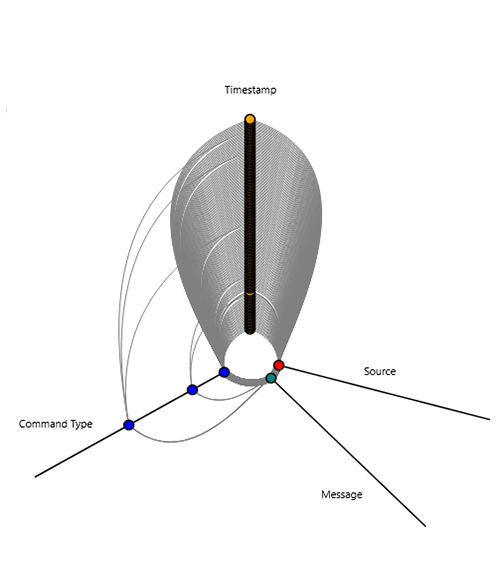
\includegraphics[width=2.5in]{images/regHive.png} 
\caption{-- Hive plot displaying a simple random sample of 150 points from the GStar Graph Database logs. Data sampled is from Feb 06, 2017 - May 25, 2017}
\label{fig:regHive}
\end{figure}

\begin{figure}[h]
\centering
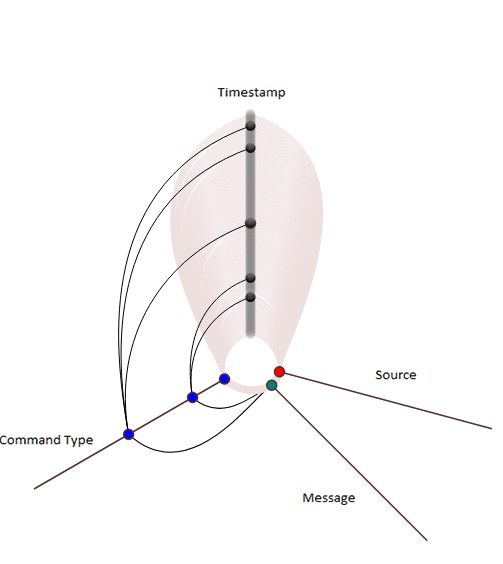
\includegraphics[width=2.5in]{images/uniqHive.png} 
\caption{-- Hive plot where the prominent nodes in the figure denote 'injections' into the GStar Graph Database that differ from normal traffic. Data sampled is from Feb 06, 2017 - May 25, 2017}
\label{fig:uniqHive}
\end{figure}

\noindent Fig. \ref{fig:XSS} displays a selected sample collected by the GStar logs between March 11, 2017 and March 16, 2017 in a hive plot. The highlighted requests range a span of 25 seconds where the XSS commands were attempted, starting with GET cgi and ending with GET ;sh\$IFS-c\$IFS'. This shows both the short amount of time it took to run this malware insertion, and the use of GET and POST request methods for one attack.

\begin{figure}[h]
\centering
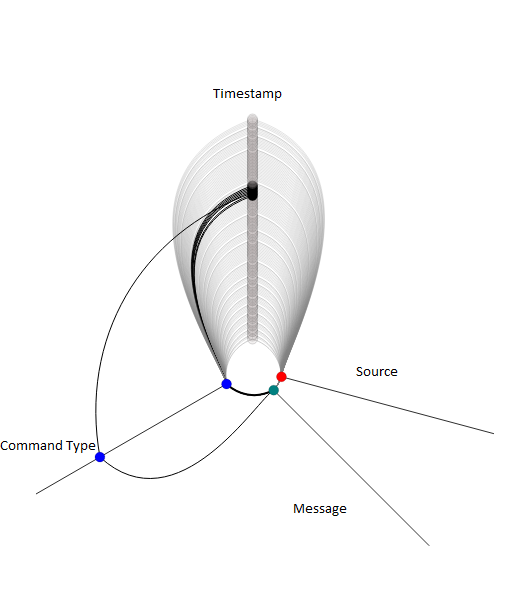
\includegraphics[width=2.5in]{images/XSS.png} 
\caption{-- Hive plot where the prominent nodes in the figure display the XSS attempt on the GStar Graph Database. Data sampled is from Mar 11, 2017 - Mar 16, 2017}
\label{fig:XSS}
\end{figure}

We determined that a very similar attack sequence was also recently documented by a Finnish cyber-security company named F-Secure \cite{F-Secure}. The commands attempted with the XSS attack are intended to upload a PHP: Hypertext Preprocessor (PHP) file, then send a series of commands that, if executed, would remove a file using the \$IFS variable found in the PHP. Afterwards, it would attempt to download a file with the same variable name and change the permissions on said file so that it can be executed by any user.  Then the attacker subsequently executes the file. Researchers from F-Secure  attribute this attack profile to a Peer to Peer (P2P) botnet named TheMoon \cite{TheMoon}. This example illustrates how we can use data collected from attack attempts to isolate and attribute the attack, provided that we can determine what types of attacks are taking place.

Pasithea was subsequently deployed, and is currently active, on an Amazon Web Services (AWS) EC2 instance in Ashburn, Virginia. Our log files indicate cursory web crawls from Baidu, a Chinese search engine, and some attempts at exploiting a known vulnerability in tomcat web servers using GET /manager/html \cite{Tomcat-Exploit}. We continue to monitor this instance, and additional results will be reported in a future paper.
